\documentclass[tikz,border=3pt]{standalone}
\usepackage[utf8]{inputenc}
\usepackage[T1]{fontenc}
\usepackage{lmodern}
\renewcommand{\familydefault}{\sfdefault}
\usepackage{sansmath}\sansmath
\usepackage{chemfig}
\usepackage{pgfplots}\pgfplotsset{compat=1.18,/pgf/number format/use comma,/pgf/number format/1000 sep={.}}
\usetikzlibrary{arrows.meta,calc,positioning,decorations.pathmorphing,patterns}
% paleta del sitio
\definecolor{nar}{HTML}{E8680C}\definecolor{narc}{HTML}{FFB35C}\definecolor{hielo}{HTML}{FFF3E8}
\definecolor{tinta}{HTML}{1D1D1F}\definecolor{gris}{HTML}{6E6E73}\definecolor{lila}{HTML}{7C5CF0}
\definecolor{azul}{HTML}{2F6FD6}\definecolor{menta}{HTML}{17A673}\definecolor{coral}{HTML}{E8342A}
\begin{document}
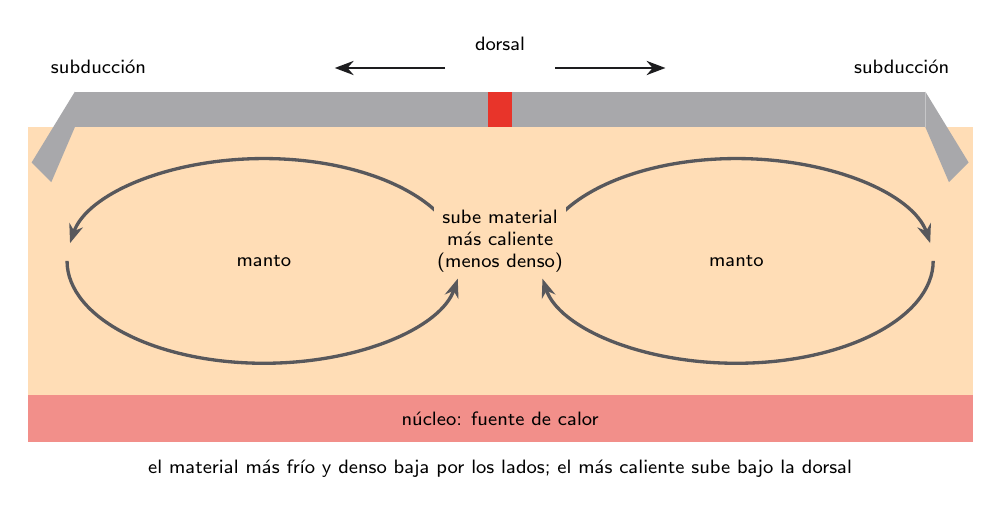
\begin{tikzpicture}[font=\footnotesize,>={Stealth[length=2.4mm]}]
% manto y nucleo
\fill[narc!45] (0,0.6) rectangle (12,4.0);
\fill[coral!55] (0,0) rectangle (12,0.6);
\node[font=\scriptsize] at (6,0.3) {núcleo: fuente de calor};
% placas
\fill[gris!60] (0.6,4.0) rectangle (5.85,4.45);
\fill[gris!60] (6.15,4.0) rectangle (11.4,4.45);
\fill[gris!60] (0.6,4.45) -- (0.6,4.0) -- (0.3,3.3) -- (0.05,3.55) -- cycle;
\fill[gris!60] (11.4,4.45) -- (11.4,4.0) -- (11.7,3.3) -- (11.95,3.55) -- cycle;
\fill[coral] (5.85,4.0) rectangle (6.15,4.45);
\draw[->,thick,tinta] (5.3,4.75) -- (3.9,4.75); \draw[->,thick,tinta] (6.7,4.75) -- (8.1,4.75);
\node[font=\scriptsize,anchor=south] at (6,4.85) {dorsal};
\node[font=\scriptsize,anchor=south] at (0.9,4.55) {subducción};
\node[font=\scriptsize,anchor=south] at (11.1,4.55) {subducción};
% celdas de conveccion
\draw[->,very thick,gris!80!black] (5.5,2.3) arc[start angle=0,end angle=170,x radius=2.5,y radius=1.3];
\draw[->,very thick,gris!80!black] (0.5,2.3) arc[start angle=180,end angle=350,x radius=2.5,y radius=1.3];
\draw[->,very thick,gris!80!black] (6.5,2.3) arc[start angle=180,end angle=10,x radius=2.5,y radius=1.3];
\draw[->,very thick,gris!80!black] (11.5,2.3) arc[start angle=0,end angle=-170,x radius=2.5,y radius=1.3];
\node[font=\scriptsize,align=center] at (3.0,2.3) {manto};
\node[font=\scriptsize,align=center] at (9.0,2.3) {manto};
\node[font=\scriptsize,align=center,fill=narc!45,inner sep=1pt] at (6,2.55) {sube material\\más caliente\\(menos denso)};
\node[font=\scriptsize,align=center,anchor=north] at (6,-0.1) {el material más frío y denso baja por los lados; el más caliente sube bajo la dorsal};
\end{tikzpicture}
\end{document}
